\documentclass[11pt,a5paper]{article}

\usepackage[T1]{fontenc}
\usepackage[utf8]{inputenc}
\usepackage{lmodern, microtype}
\usepackage[estonian]{babel}

\usepackage{siunitx}
\sisetup{inter-unit-product=\ensuremath{{}\cdot{}}, per-mode=fraction, exponent-product=\cdot, output-decimal-marker={,}}

\usepackage{graphicx}
\usepackage{wrapfig}
\usepackage{subfig}
\usepackage{tikz}
\usetikzlibrary{patterns, patterns.meta}
\usetikzlibrary{arrows.meta}
\usepackage[european]{circuitikz}
\tikzset{component/.style={draw,thick,circle,fill=white,minimum size=0.75cm,inner sep=0pt}}
\usepackage{amsmath,amssymb}
\usepackage{amsfonts}
\usepackage[hidelinks]{hyperref}
\usepackage{csquotes}
\usepackage{caption}
\usepackage{enumitem}
\usepackage{wrapfig}
\topmargin=-3.0cm \textheight=19cm \textwidth=12.9cm
\oddsidemargin=-1.5cm  \evensidemargin=-1.5cm
\setlength{\parindent}{0pt} \setlength{\parskip}{6pt} \sloppy
\sloppy \relpenalty=10000 \binoppenalty=10000
\pagestyle{empty}

\newcommand{\numb}[1]{\vspace{5pt}\textbf{\large #1}}
\newcommand{\nimi}[1]{(\textsl{\small #1})}
\newcommand{\punktid}[1]{(\emph{#1~p.})}
\newcounter{ylesanne}
\newcommand{\yl}[1]{\addtocounter{ylesanne}{1}\numb{\theylesanne.} \nimi{#1} \newblock{}}
\newcommand{\autor}[1]{}% Kasuta võistluse ajal
%\newcommand{\autor}[1]{\emph{ Autor: #1}}% Kasuta kui vaja autorit

\begin{document}
\begin{center}
  \textbf{\Large Eesti koolinoorte 33.\ füüsika lahtine võistlus} \par
  \emph{3.\ detsember 2022. a.\\Vanema rühma ülesanded (11.--12.\ klass)}
\end{center}

\resizebox{\textwidth}{!}{
  \emph{%
    \begin{tabular}{@{}l@{}}
      \textbf{Palun kirjutada iga ülesande lahendus eraldi lehele.}\\
      Lahendamisaeg on 5 tundi. \\
      Iga osavõtja võib lahendada kõiki pakutud ülesandeid. \\
      Arvesse lähevad 6 suurima punktide arvu saanud lahendust. \\
      Kasutada võib kirjutus- ja joonestusvahendeid ning kalkulaatorit. Muud abivahendid on keelatud.\\
    \end{tabular}
  }
} \par



\yl{TITICACA JÄRV}
Titicaca järvest Boliivia ja Peruu piiril voolab ainsa jõena välja Desaguadero jõgi kiirusega $v=\SI{10}{\meter\cubed\per\second}$. Järve pindala on $S=\SI{8400}{\kilo\meter\squared}$ ja keskmine vee aurustumise kiirus järve pinnalt on aastas $b=\SI{2000}{\milli\meter}$. 

Leidke Titicaca järve soolsus kui sissetuleva vee soolsus on $c=\SI{10}{\milli\gram\per\liter}$. Eeldage, et järves on soola kontsentratsioon ja veetase igal ajahetkel ühtlased.
\punktid{6} \autor{Kaur Aare Saar}



\begin{wrapfigure}{r}{0.1\textwidth}
\raisebox{3pt}[\dimexpr\height-0.6\baselineskip\relax]{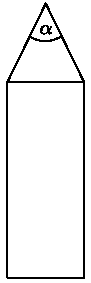
\includegraphics[scale=0.95]{pliiats_joonis.pdf}}
\vspace{-55pt}
\end{wrapfigure}
\yl{PLIIATS}
Pliiatsi kahe näpu vahel õhus hoidmiseks tuleb rakendada sama jõudu olenemata sellest, kas hoitakse kinni tipust või külje pealt. Näpu hõõrdetegurid pliiatsi küljega ja teritatud osaga on vastavalt $\mu_1 = \SI{0,3}{}$ ja $\mu_2 = \SI{0,5}{}$. Milline on pliiatsi tipunurk $\alpha$?
\punktid{8} \autor{Joonas Kalda}


\begin{wrapfigure}{r}{0.16\textwidth}
\raisebox{-5pt}[\dimexpr\height-0.6\baselineskip\relax]{
  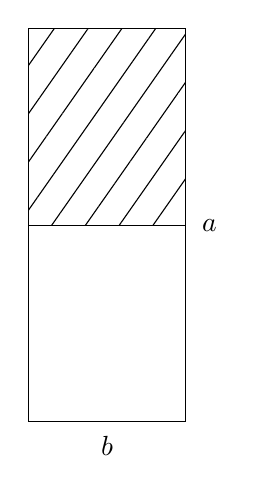
\begin{tikzpicture}
    \draw (0,0) rectangle (2,2.5);
    \draw[pattern={Lines[angle=55,distance=10pt]}] (0,2.5) rectangle (2,5);
    \draw (2.3,2.5) node {$a$};
    \draw (1,-0.3) node {$b$};
  \end{tikzpicture}
}
\end{wrapfigure}

\yl{KÕND ESKALAATORIL} 
Sandra eesmärk on kõndida ristkülikukujulise koridori alumisest vasakust nurgast ülemisse paremasse nurka. Koridor on piklik ristkülik  (pealtvaade joonisel) pikkusega $a = \SI{200}{m}$ ja laiusega $b = \SI{4}{m}$. Enda aitamiseks saab ta koridori ülemise poole põranda asendada vabalt valitud suunas liikuva lindiga (nagu tihti lennujaamades olevad horisontaalsed eskalaatorid). Sandra soovib lindi liikumissuuna valida selliselt, et ta saab võimalikult kiiresti koridori alumisest vasakust nurgast koridori ülemisse paremasse nurka jõuda. Millise nurga all koridori vasakpoolse küljega peaks Sandra lindi liikumissuuna valima? Sandra kõnnib enda all oleva pinna suhtes maksimaalse kiirusega $v = \SI{2}{\meter \per \second}$, lint liigub maksimaalse kiirusega $u = \SI{3}{\meter \per \second}$.\\
\emph{Märkus:} kui $x \approx 0$, siis võib kasutada lähendusi $\sqrt{1+x} \approx 1 + \frac{x}{2}$ ja $\sin{x} \approx \tan{x} \approx x$ (nurk $x$ on radiaanides).
\punktid{8} \autor{Kaarel Hänni}

\newpage



\yl{KUIV JÄÄ}
Kuiva jääd (tahke CO\(_{2}\) ) kasutatakse vahel, et tekitada sublimeerumisel eraldunud gaasi ning veepiiskade abil madal udu näiteks teatris või võtteplatsil. Noor füüsik Gerda tahab teada, mis sellisel tegevusel juhtuks kinnises ruumis. Selleks võtab ta natuke kuiva jääd (\(m_{CO_2}\) = \SI{10}{\gram}) sublimeerumistemperatuuril (\(T_{0}\) = \SI{-78,5}{\degreeCelsius}) ja asetab selle tühja tünni diameetriga \(D\) = \SI{1}{\meter} ja kõrgusega \(h\) = \SI{1,5}{\metre}. Gerda sulgeb tünni koheselt ja jätab meelde, et koos jääga on seal sees toatemperatuuril (\(T_{\textup{õhk}}\) = \SI{25}{\degreeCelsius}) õhk. Eeldame, et tünni seinade soojusmahtuvus on tühine ning ei toimu soojusvahetust tünnivälise keskkonnaga.
\\(a) Milline on õhutemperatuur ning -rõhk tünnis siis, kui kogu kuiv jää on sublimeerunud?
\\(b) Kuidas ja miks muutuksid (suureneks, väheneks, jääks samaks) õhutemperatuur ning -rõhk, kui Gerda oleks kuiva jää pannud tünni põhja veevanni, nagu seda tihti kasutatakse?\\
Kuiva jää sublimeerumissoojus on \(\lambda_{CO_2}\) = \SI{32,3}{\kilo\joule\per\mole}. Süsiniku ja hapniku molaarmassid on vastavalt \(M_C\) = \SI{12,0}{\gram\per\mole} ja \(M_O\) = \SI{16,0}{\gram\per\mole}. Õhu tihedus toatemperatuuril on \(\rho_{\textup{õhk}}\) = \SI{1,29}{\kilo\gram\per\metre\cubed}. Süsihappegaasi ja õhu erisoojusmahtuvused konstantsel ruumalal on vastavalt \(C_{CO_{2}}\) = \SI{0,657}{\kilo\joule\per\kelvin\per\kilo\gram} ja \(C_{\textup{õhk}}\) = \SI{0,718}{\kilo\joule\per\kelvin\per\kilo\gram}. Atmosfäärirõhk on \(p_{0}\) = \SI{101,3}{\kilo\pascal} ning universaalne gaasikonstant R = \SI{8,314}{\joule\per\kelvin\per\mole}.
\punktid{8} \autor{Uku Andreas Reigo}





\begin{wrapfigure}{r}{0.25\textwidth}
\raisebox{0pt}[\dimexpr\height-0.6\baselineskip\relax]{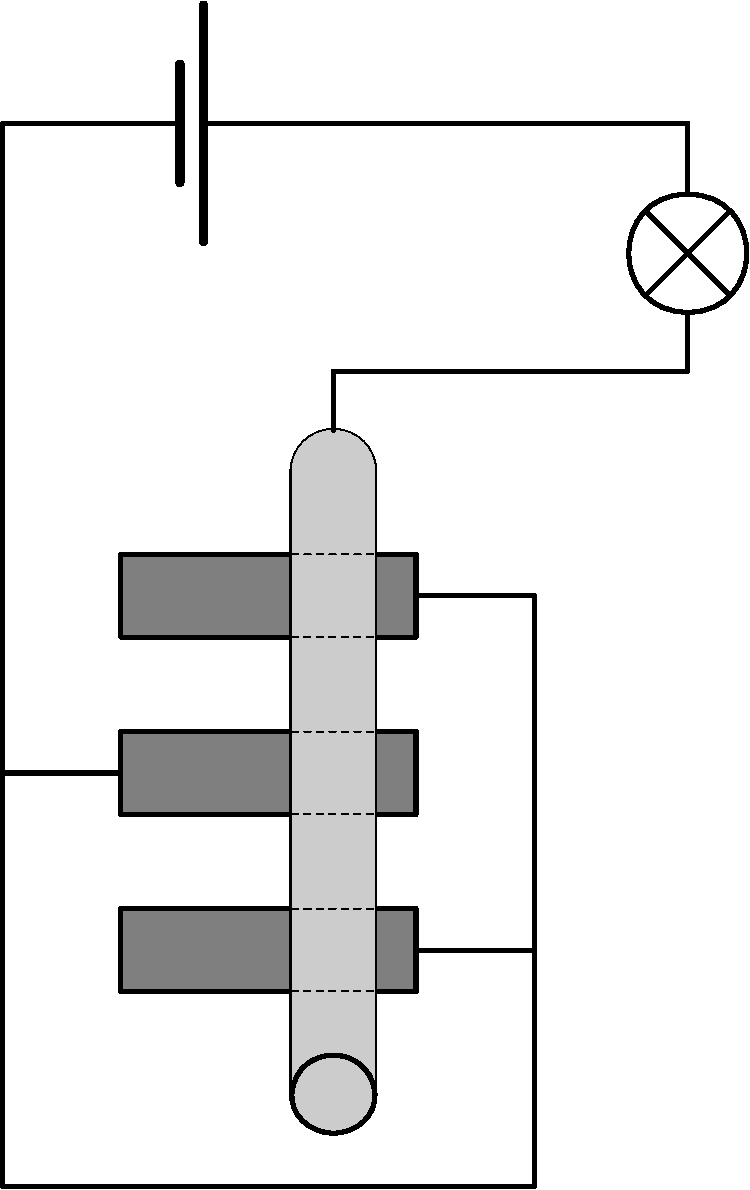
\includegraphics[scale=0.25]{reostaadid.pdf}}
\end{wrapfigure}


\yl{ORIGINAALSED REOSTAADID}
Õhukeste grafiitplaatide mõõtmed on 100 $\mu$m $\times$ 1 cm $\times$ 10 cm ning eritakistus on $\rho =  \SI{1}{\Omega m}$. Kolm sellist plaati paiknevad paralleelselt isolaatoril ja igale neist on ühele otstest ühendatud plaadilaiune klemm (ei pea olema tingimata kõigil samas otsas!). Kõik need kolm klemmi on juhtmetega ühendatud patarei ühe otsaga. Patarei teine ots on ühendatud $R = \SI{10}{k \Omega}$ takistust omava tarbija ühe klemmiga. Selle tarbija teine klemm on ühendatud juhtmete kaudu juhist toruga, mis on paigutatud risti üle kõigi kolme paberilipaka nagu näidatud joonisel. Patarei elektromotoorjõud $U =\SI{12}{V}$ ja sisetakistus on tühine.
\\(a) Kui toru puudutab kõiki pabereid $l = \SI{8}{cm}$ nende vasakust otsast, siis rakendub tarbijal ligikaudu võimsus $P = \SI{2,65}{mW}$. Mitu plaati on ühendatud vasakult? 
\\(b) Milline võimsus rakenduks tarbijal, kui liigutada toru nii, et ta puutuks iga paberilipakat vasakust otsast \SI{7}{cm} kauguselt.
\punktid{10} \autor{Richard Friedrichs}


\newpage


\yl{SAUN}
Subjektiivset palavusetunnet kuumas õhus kirjeldab väga hästi see, kui palju erineb kastepunkt keha temperatuurist. Kastepunkt on temperatuur, mille juures antud õhust hakkab vesi välja kondenseeruma (eeldusel, et rõhk püsib võrdne atmosfäärirõhuga). Olgu leiliruumi õhutemperatuur $T_l=\SI{100}{\celsius}$, saunaõhu kastepunkt $T_k=\SI{10}{\celsius}$ ja leiliruumi ruumala $V=\SI{10}{m^3}$. Mitme kraadini kerkib kastepunkt, kui leiliks vistakase $m=\SI{200}g$ vett? Universaalne gaasikonstant $R=\SI{8.31}{\joule\per\kelvin\per\mole}$; vee molaarmass $\mu=\SI{18}{\gram \per \mole}$.
\punktid{10} \autor{Jaan Kalda}
\begin{center}
    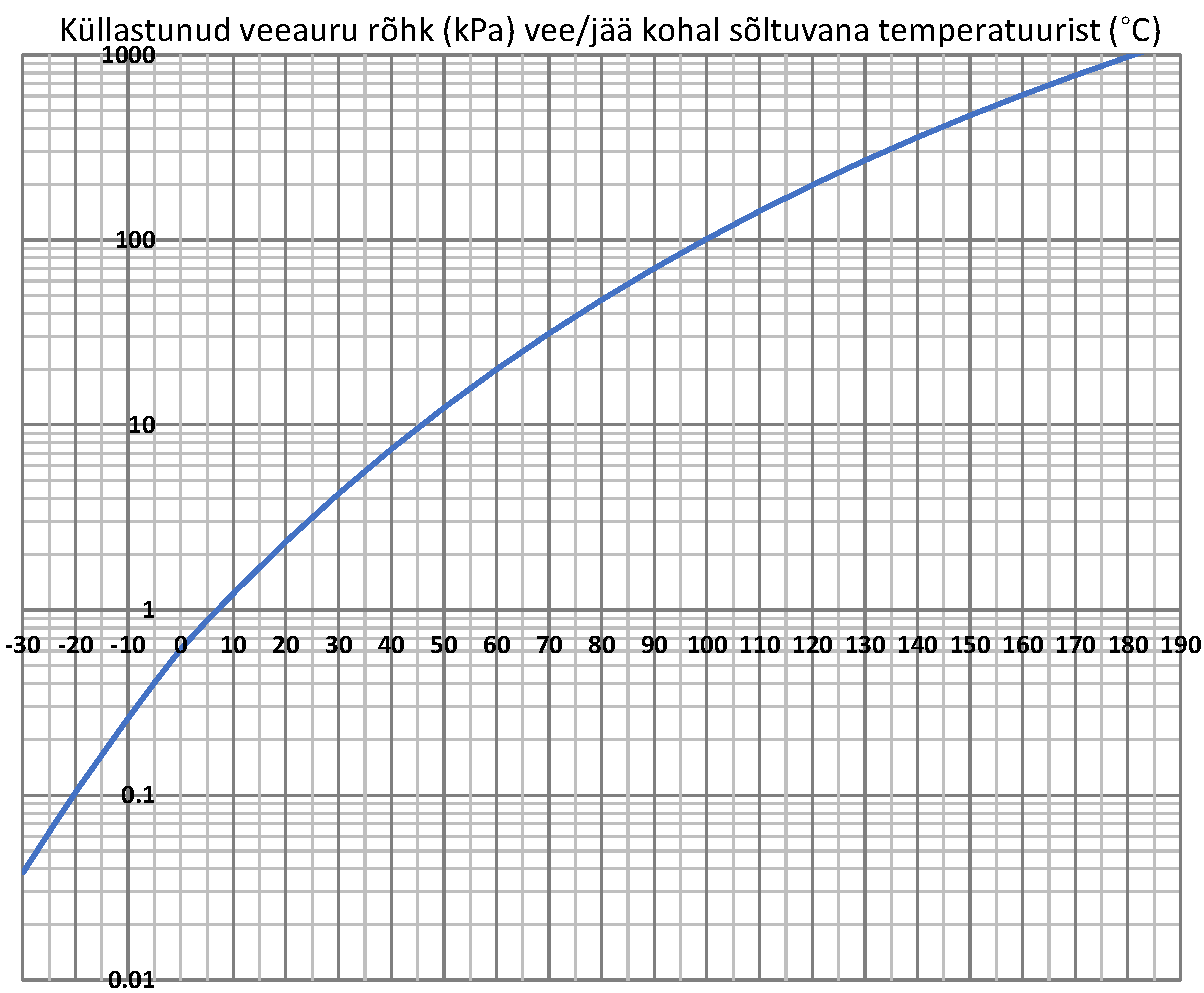
\includegraphics[width=\textwidth]{veeaur_.pdf}
\end{center}



\yl{ELEKTRON JA KONDENSAATOR} Plaatkondensaatori plaadid on ruudukujulised küljepikkusega $b$ ja plaatide vahekaugus $d$ on hulga väiksem kui $b$; plaatide vahele on rakendatud pinge $U$. Millist minimaalset algkiirust $v$ peab omama elektron massiga $m$ ja laenguga $e$, et see suudaks läbida plaatide vahelise ruumi ilma vastu plaate põrkamata? Elektron peab väljuma plaatidevahelisest ruumist sisenemispunkti suhtes vastasküljelt.
\punktid{10} \autor{Jaan Kalda}

\newpage

\yl{KAUBALAEV} Lastimise käigus hakkab kaubalaev tasases vees väikse amplituudiga üles-alla võnkuma. Kui laevale on tõstetud $m_1 = \SI{1000}{}$ tonni kaupa, on võnkumiste sagedus $f_1 = \SI{10}{}$ võnget minutis. Kui laevale on tõstetud $m_2 = \SI{10000}{}$ tonni kaupa, on võnkumiste sagedus $f_2 = \SI{8}{}$ võnget minutis. On teada, et laeva võnkumine haarab kaasa ka teatud hulga vett, mis näiliselt suurendab laeva inertsi. See tähendab, et vees reageerib laev välisjõududele nii, nagu oleks tema mass kaasahaaratud vee massi võrra tegelikust suurem. Leida laeva tühimass $M$ arvestades, et sõltumata kauba hulgast on kaasahaaratud vee mass $\frac{1}{2}M$. Eeldage, et veepinna lähedal on laeva kere väliskülg vertikaalne.
\punktid{10} \autor{Päivo Simson}



\yl{NURK}
Spioonil on kodus koer, kellel ta tahab spioneerimise harjutamiseks alati silma peal hoida. Kodus on koridor, mille keskel on nurk suurusega $\alpha$, mille taha vastu seina koer mõnikord konutama läheb. Spioonile meeldib aga konutada teisel pool nurka, samuti vastu seina. Spioonil on selliste puhkude jaoks kumerlääts fookuskaugusega $f=\SI{10}{cm}$, mis on kettakujuline raadiusega $r=\SI{5}{cm}$, mille ta saab asetada koridoris vabalt valitud kohta, vabalt valitud orientatsiooniga. Milline on minimaalne nurk $\alpha$, mille puhul on spioonil võimalik läätse kasutades koera antud situatsioonis jälgida?\\
\emph{Märkus:} võib eeldada, et nii spiooni kui koera kaugus nurgast on palju suuremad kui nende mõõtmed, mis on omakorda palju suuremad kui läätse raadius. Läätse võib vaadelda ideaalse õhukese läätsena.
\punktid{12} \autor{Kaarel Hänni}

\begin{wrapfigure}{r}{0.45\textwidth}
\raisebox{0pt}[\dimexpr\height-0.6\baselineskip\relax]{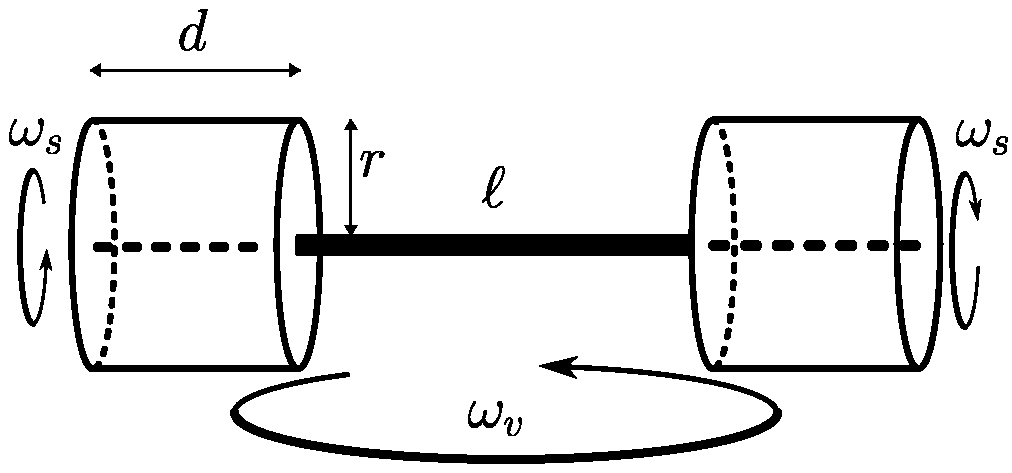
\includegraphics[scale=0.37]{hantel_joonis.pdf}}
\vspace{-15pt}
\end{wrapfigure}
\yl{HANTEL JA PÖÖRLEMINE}
Hantel koosneb kahest ühesugusest silindrist raadiusega $r$ ning kõrgusega $d$, mis on ühendatud koaksiaalselt vardaga pikkusega $l$. Varda sees on mootor, mis pöörab silindreid varda suhtes võrdsete ja vastassuunaliste nurkkiirustega $\pm \omega_s$. Millise püsiva nurkkiiruse $\omega_v$ omandab varras, kui hantel asetatakse siledale horisontaalpinnale? Eeldada, et varras ei hakka pöörlema ümber oma telje (nt saab seda takistada kinnitades varda keskkohast alla rippuva lisaraskuse).
\punktid{12} \autor{Marko Tsengov}

\end{document}
